\documentclass[
  bibliography=totoc,     % Literatur im Inhaltsverzeichnis
  captions=tableheading,  % Tabellenüberschriften
  titlepage=firstiscover, % Titelseite ist Deckblatt
  12pt,
]{scrartcl}

% Paket float verbessern
\usepackage{scrhack}

% Warnung, falls nochmal kompiliert werden muss
\usepackage[aux]{rerunfilecheck}

% unverzichtbare Mathe-Befehle
\usepackage{amsmath}
% viele Mathe-Symbole
\usepackage{amssymb}
% Erweiterungen für amsmath
\usepackage{mathtools}
% Zeilenabstand zu 1,5 
\usepackage[onehalfspacing]{setspace}

\usepackage[% Seitenlayout anzeigen
  left=2.5cm,
  right=2.5cm,
  top=3.5cm,
  bottom=3.5cm,
  %includeheadfoot
]{geometry}

% Fonteinstellungen zu TNR
%\usepackage{fontspec}
%\setmainfont{Times New Roman}
%
%% Don't use \fontspec directly to change the font
%
%\newfontfamily\subsubsectionfont{Times New Roman}
%\newfontfamily\subsectionfont{Times New Roman}
%\newfontfamily\sectionfont{Times New Roman}
%
%% Set formats for each heading level
%\setkomafont{disposition}{\sectionfont\bfseries}
%%\setkomafont{normalfont}{\sectionfont}
%\addtokomafont{title}{\Large\bfseries\sectionfont}
%\addtokomafont{subtitle}{\large\bfseries\sectionfont}
%\addtokomafont{section}{\Large\bfseries\sectionfont}
%\addtokomafont{subsection}{\large\bfseries\subsectionfont}
%\addtokomafont{subsubsection}{\large\subsubsectionfont}
%\addtokomafont{subsubsection}{\large\bfseries\subsubsectionfont}

% Latin Modern Fonts werden automatisch geladen
% Alternativ zum Beispiel:
%\setromanfont{Libertinus Serif}
%\setsansfont{Libertinus Sans}
%\setmonofont{Libertinus Mono}

% Wenn man andere Schriftarten gesetzt hat,
% sollte man das Seiten-Layout neu berechnen lassen
%\recalctypearea{}

% deutsche Spracheinstellungen
\usepackage{polyglossia}
\setmainlanguage{german}


\usepackage[
  math-style=ISO,    % ┐
  bold-style=ISO,    % │
  sans-style=italic, % │ ISO-Standard folgen
  nabla=upright,     % │
  partial=upright,   % ┘
  warnings-off={           % ┐
    mathtools-colon,       % │ unnötige Warnungen ausschalten
    mathtools-overbracket, % │
  },                       % ┘
]{unicode-math}

% traditionelle Fonts für Mathematik
\setmathfont{Latin Modern Math}
% Alternativ zum Beispiel:
%\setmathfont{Libertinus Math}

\setmathfont{XITS Math}[range={scr, bfscr}]
\setmathfont{XITS Math}[range={cal, bfcal}, StylisticSet=1]

% Zahlen und Einheiten
\usepackage[
  locale=DE,                   % deutsche Einstellungen
  separate-uncertainty=true,   % immer Fehler mit \pm
  per-mode=symbol-or-fraction, % / in inline math, fraction in display math
]{siunitx}

% chemische Formeln
\usepackage[
  version=4,
  math-greek=default, % ┐ mit unicode-math zusammenarbeiten
  text-greek=default, % ┘
]{mhchem}

% richtige Anführungszeichen
\usepackage[autostyle]{csquotes}

% schöne Brüche im Text
\usepackage{xfrac}

% Standardplatzierung für Floats einstellen
\usepackage{float}
\floatplacement{figure}{htbp}
\floatplacement{table}{htbp}

% Floats innerhalb einer Section halten
\usepackage[
  section, % Floats innerhalb der Section halten
  below,   % unterhalb der Section aber auf der selben Seite ist ok
]{placeins}

% Seite drehen für breite Tabellen: landscape Umgebung
\usepackage{pdflscape}

% Captions schöner machen.
\usepackage[
  labelfont=bf,        % Tabelle x: Abbildung y: ist jetzt fett
  font=small,          % Schrift etwas kleiner als Dokument
  width=0.9\textwidth, % maximale Breite einer Caption schmaler
]{caption}
% subfigure, subtable, subref
\usepackage{subcaption}

% Grafiken können eingebunden werden
\usepackage{graphicx}
% größere Variation von Dateinamen möglich
\usepackage{grffile}

% schöne Tabellen
\usepackage{booktabs}

% Verbesserungen am Schriftbild
\usepackage{microtype}

% Literaturverzeichnis
\usepackage[
  backend=biber,
]{biblatex}
% Quellendatenbank
\addbibresource{lit.bib}
\addbibresource{programme.bib}

% Hyperlinks im Dokument
\usepackage[
  unicode,        % Unicode in PDF-Attributen erlauben
  pdfusetitle,    % Titel, Autoren und Datum als PDF-Attribute
  pdfcreator={},  % ┐ PDF-Attribute säubern
  pdfproducer={}, % ┘
]{hyperref}
% erweiterte Bookmarks im PDF
\usepackage{bookmark}

% Trennung von Wörtern mit Strichen
\usepackage[shortcuts]{extdash}

\author{%
  Max Koch\\%
  \href{mailto:max.koch@udo.edu}{max.koch@udo.edu}\\%
  \\%
  \small{Projektpartner: Johannes Lamers}\\%
  \small{\href{mailto:johannes.lamers@tu-dortmund.de}{johannes.lamers@tu-dortmund.de}}%
}
\publishers{TU Dortmund – Fakultät Physik}


\title{Machinelles Lernen für Physiker}
\subtitle{Genre Erkennung von Kunstwerken}
\date{%
  09.08.2021
}

\begin{document}

\maketitle
\thispagestyle{empty}
{\renewcommand*\normalfont{\usekomafont{disposition}}%
\normalfont%
\tableofcontents}
\newpage
% \onehalfspacing

\section{Motivation}
Kunst war schon immer ein großer Teil der Menschheitsgeschichte.
Durch Gemälde öffnet sich für den Betrachter*in eine Tür in die Gedanken des Künstlers*in.
Diese spiegeln sich besonders durch die verschiedenen Motive, die Künstler*in auf ihren Bildern verewigt haben wieder.
Aber auch die Darstellungsweise gibt einen Eindruck von der Zeit in der das Bild entstanden ist und aus welchem Umfeld der Künstler*in stammt.
So liegt es nur Nahe Bilder entsprechend ihre Motive, Darstellungsweise und nach ihrem Schaffungszeitpunkt zu kategorisieren.
In der Kunst werden diese Kategorien Genre oder Gattung genannt.
\\\\
Oft ist es allerdings schwer für den Laien*in die Einordnung eines Kunstwerkes in sein Genre selbstständig zu machen.
Denn einige Genre werden nur durch wenige Details von einem anderen Genre getrennt.
Teilweise verschwimmen diese Grenzen sogar komplett, wodurch dem Gemälde mehrere Genres zugesprochen werden können.
Es ist aber für das Verständnis und die Interpretation des Gemäldes essenziell das Genre des Bildes zu kennen.
Um die Kunst für Laien*in zugänglicher zu machen wird deshalb folgende Frage gestellt:
\\
\textbf{Ist es möglich das Genre eines Gemäldes durch das Einlesen des Bildes in ein Convolutional Neural Network (CNN) zu bestimmen?}
\\
Dies würde es dem Laien*in ermöglichen einfach das Genre eines Kunstwerkes zu erfahren und ihm so ein besseres Erlebnis beim Genuss der Kunst bieten.
Dabei haben wir uns zunächst auf einen Datensatz beschränkt, auf diesen wird im folgenden weiter eingegangen.

\section{Charakterisierung des Datensatzes}
\label{sec:Charakterisierung}
Der genutzte Datensatz stammt von der Website \href{https://www.kaggle.com/}{kaggle}.
Diese ist eine Website auf der Datensätze geteilt werden können.
Dies ermöglicht es den Nutzern*innen diese zu analysieren oder zum Beispiel damit ein Neuronales Netzwerk zu trainieren.
\\\\
Der genutzte Datensatz trägt den Namen \href{https://www.kaggle.com/ikarus777/best-artworks-of-all-time}{Best Artworks of All Time}.
Es wurde dieser Datensatz gewählt, da in dem Datensatz viele bekannte Gemälde enthalten sind.
Zudem deckt der Datensatz eine große Spanne an bekannten Genre und Künstlern ab.
So gibt er eine gute Stichprobe an Bildern von bekannten Genre.
%Die Bilder des Datensatzes wurden von dem Ersteller des Datensatzes von der Website \href{http://artchallenge.ru/?lang=en}{artchallenge.ru} kopiert.
Der Datensatz besteht dabei aus drei Datein.
\\
Einer "artists.csv"-Datei in der die Namen, und die Genre der Kunstwerke der Künstler*innen gespeichert sind.
In der "artists.csv"-Datei sind zudem einige weitere Daten wie zum Beispiel die Nationalität der Künstler*innen zu finden.
Diese Daten werden allerdings nicht für das Neuronale Netzwerk genutzt, da explizit nur aus den Bildern selber das Genre des Bildes ermittlet werden soll.
Die im Datensatz enthaltenen Künstler*innen sind in Tabelle \ref{tab:artist} im Anhang \ref{sec:anhang} zu finden.
Zudem sind in der Tabelle die Genre, die den Gemälde der Künstler*innen zugeordnet werden und die Anzahl der Bilder des Künstlers*in im Datensatz zu finden.
In Summe beinhaltet der Datensatz 8446 Bilder von 50 verschiedenen Künstlern*innen.
\\
Des weiteren besteht der Datensatz aus einem "images.zip"-Ordner in dem alle Bilder in voller Auflösung gespeichert sind.
Dabei befinden sich im "images.zip"-Ordner 50 weitere Ordner.
Die Ordner tragen jeweils den Namen von einem der Künstler*innen und beinhalten alle Bilder des jeweilgen Künstlers*in die in dem Datensatz vorhanden sind.
\\
Der letzte Teil des Datensatz ist der "resized.zip"-Ordner.
In diesem befinden sich ebenfalls alle Bilder allerdings ohne die Ordner Struktur von "images.zip" und die Größe der Bilder wurde bereits geändert.
Aus diesem Grund ist der "resized.zip"-Ordner ebenfalls irrelevant für den weiteren Verlauf.
\\\\
Einige Beispiel Bilder sind in Abbildung \ref{fig:bilder_datensatz} zu sehen.
In diesem Fall ist deutlich zu erkennen, dass die Bilder unterschiedlichen Genre angehören, diese Unterscheidung ist allerdings nicht immer so einfach.
Ein Beispiel für Bilder bei denen es schwer ist das Genre zu bestimmen wird im Verlauf des Abschnitts \ref{sec:ergebnisse} gezeigt.
\begin{figure}
    \centering
    \caption{Drei Beispiel Bilder aus drei verschiedenen Genre von bekannten Künstlern.}
    \begin{subfigure}{0.30\textwidth}
        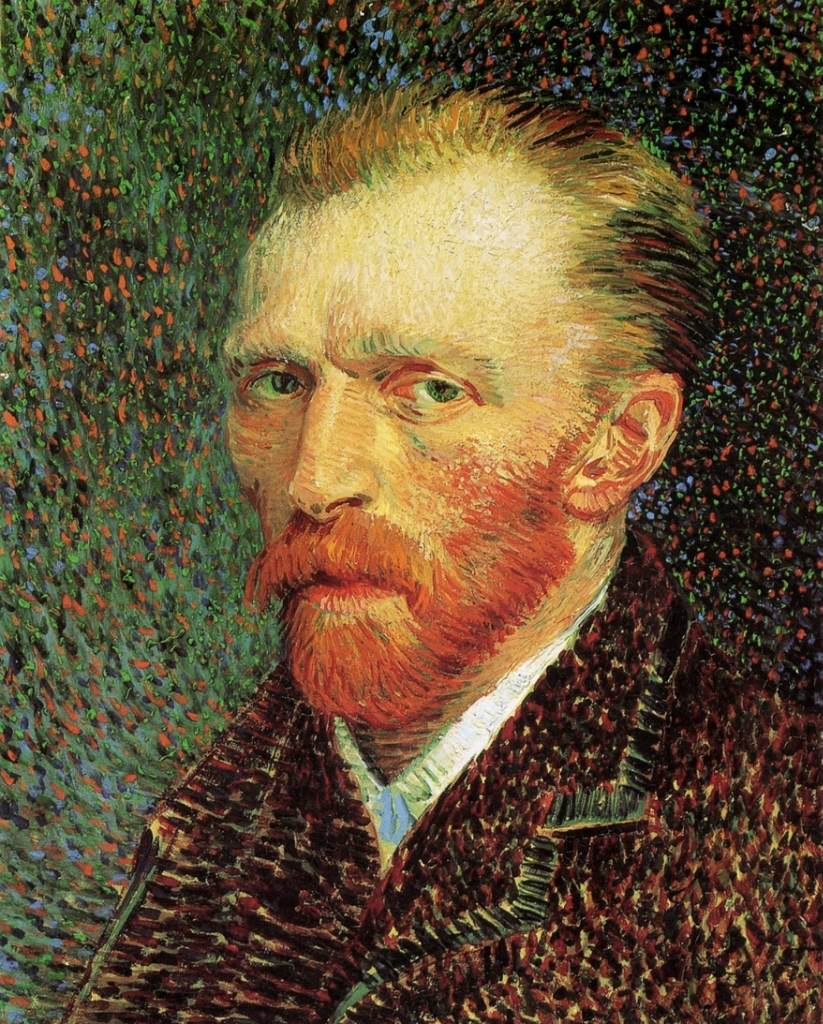
\includegraphics[width=\linewidth]{content/data/Vincent_van_Gogh_582.jpg}
        \caption{"Selbstbildnis", Vincent van Gogh 1887, Öl auf Karton, Post-Impressionismus}
        \label{fig:6}
    \end{subfigure}\hfil % <-- added
    \begin{subfigure}{0.30\textwidth}
      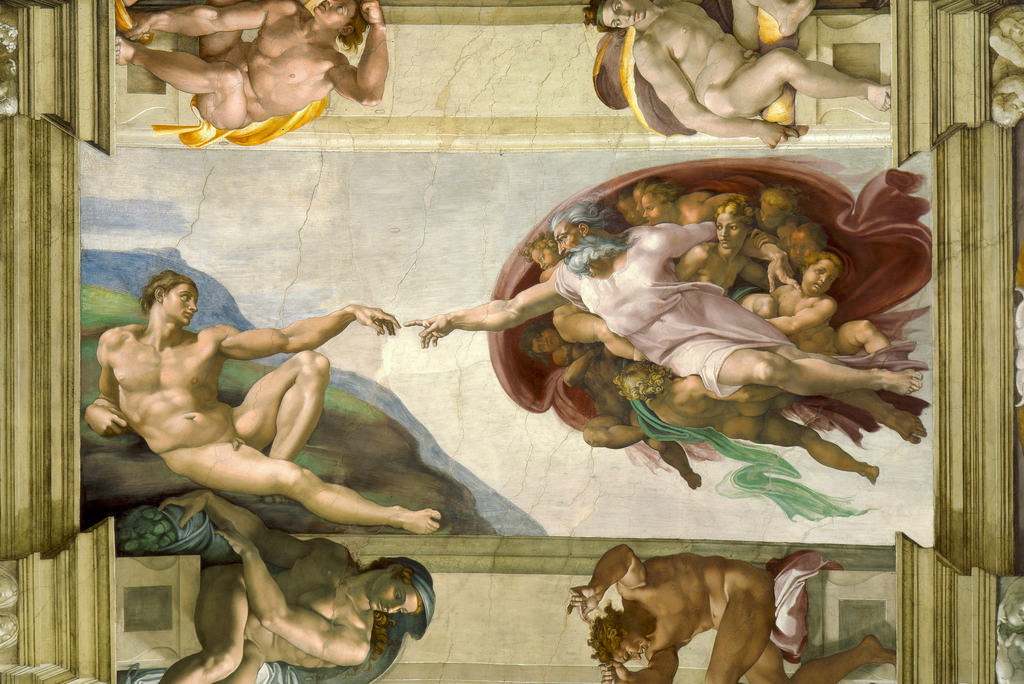
\includegraphics[width=\linewidth]{content/data/Michelangelo_4.jpg}
      \caption{"Die Erschaffung Adams", Michelangelo zwischen 1508 und 1512, ein Fresko in der Sixtinischen Kapelle, Hochrenaissance}
      \label{fig:2}
    \end{subfigure}\hfil % <-- added
    \begin{subfigure}{0.30\textwidth}
      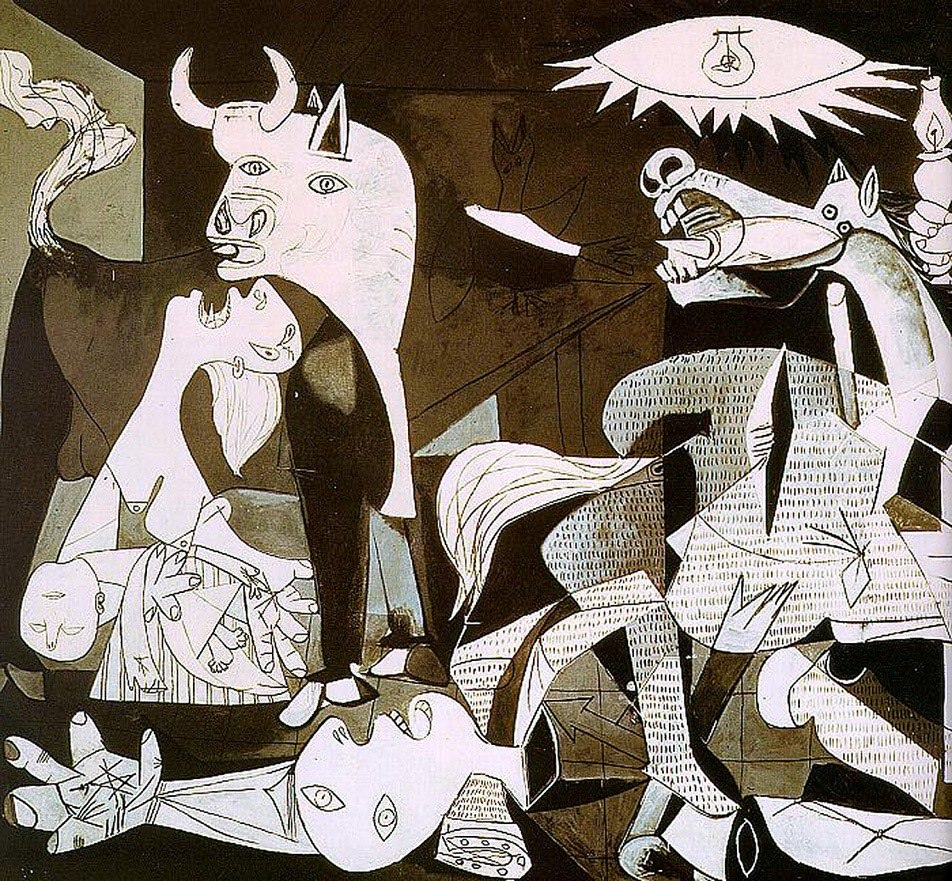
\includegraphics[width=\linewidth]{content/data/Pablo_Picasso_270.jpg}
      \caption{"Guernica", Pablo Picasso 1937, Öl auf Leinwand, Ausschnitt des Orginals, Kubismus}
      \label{fig:4}
    \end{subfigure}\hfil % <-- added
    \label{fig:bilder_datensatz}
\end{figure}
\section{Herangehensweise und Lösungsansatz}
\label{sec:loesungsansatz}
Um den Bildern des "images.zip"-Odners ihr Genre zuzuordnen wurde zunächst die "artists.csv"-Datei modifiziert.
Da diese die Information über die Genre eines Künstlers*in trägt ist es möglich durch sie den Bildern ihr Genre zuzuordnen.
Allerdings haben einige der Künstler*innen Bilder aus verschiedenen Genre geschaffen, weshalb in der "artists.csv"-Datei mehrere Genre unter ihrem Namen zu finden sind.
Da es alledings schwierig wäre den einzelnen Bildern der betroffenen Künstlern*innen das richtige Genre zuzuordnen, wurden jedem betroffenen Künstler*in nur ein Genre zugewiesen.
Dabei wurde das Genre welches dem Künstler*in letztendlich zugewiesen wurde zufällig aus den Genre des Künstlers*in gewählt.
Da allerdings die meisten Künstler*innen im Datensatz nur Bilder eines Genre geschaffen haben ist es nur in 12 von 50 Künstlern*innen dazu gekommen das Genre gestrichen wurden.
Die neue Datei die für jeden Künstler*in nur noch ein Genre enthält wurde "artist\_cut.csv" genannt.
Die Bilder der betroffenen Künstler*innen wurden dabei nicht verändert oder gelöscht.
\\\\
Um ein besseres Gefühl für den Datensatz zu bekommen wurde zunächst ein Jupyter Notebook \cite{Kluyver2016jupyter} erstellt in welches die "artists\_cut.csv" eingelesen wurde.
In diesem wurden nun die Anzahl der Bilder pro Genre bestimmt.
Die eingelesene Datei enthält 22 verschiedene Genre mit sehr unterschiedlicher Anzahl von Gemälden pro Genre.
Dieser Unterschied in der Anzahl von Bildern pro Genre  würde im Neuronalen Netzwerk zu einem ungleich verteilten Lernen führen.
Deshalb wurden aus dem Datensatz zunächst alle Bilder entfernt die Teil eines Genre sind welches nur 200 oder weniger Bilder beinhaltet.
Nach dem entfernen dieser Bilder bleiben noch 7343 Bilder aus 12 Genre.
\\\\
Nun wurde ein neuer Ordner erstellt in dem sich 12 weitere Ordner befinden.
Diese wurden nach den 12 Genre benannt die nach dem Aussortieren geblieben sind.
Danach wurden alle Bilder des jeweiligen Genre in den zugehörigen Ordner kopiert.
Der so erstellte Ordner "images\_genre.zip" wurde anschließend in ein neues Jupyter Notebook eingelesen.
Die Bilder wurden mit dem \textit{ImageDataGenerator} der Bibliothek \textit{Tensorflow} \cite{tensorflow2015-whitepaper} eingelesen und auf eine Größe von $100 \times 100 \times 3$ Pixeln gebracht.
Da der \textit{ImageDataGenerator} einen "Iterator" erstellt und es für uns intuitiver war mit arrays zu arbeiten haben wir darauf den Inhalt des Iterators in eine $X$ Matrix und einen $y$ Vektor überschrieben.
In der $X$ Matrix befinden sich dabei die quadratischen Bilder im RGB Format.
Der $y$ Vektor ist ein "One-Hot-Vector" auf deutsch ein "1-aus-n-Vektor".
Einige Beispiel für die verarbeiteten Bilder, die in der selben Form dem Neuronalen Netzwerk übergeben wurden, sind in Abbildung \ref{fig:beispiel_bilder} zu finden.
\begin{figure}
    \centering
    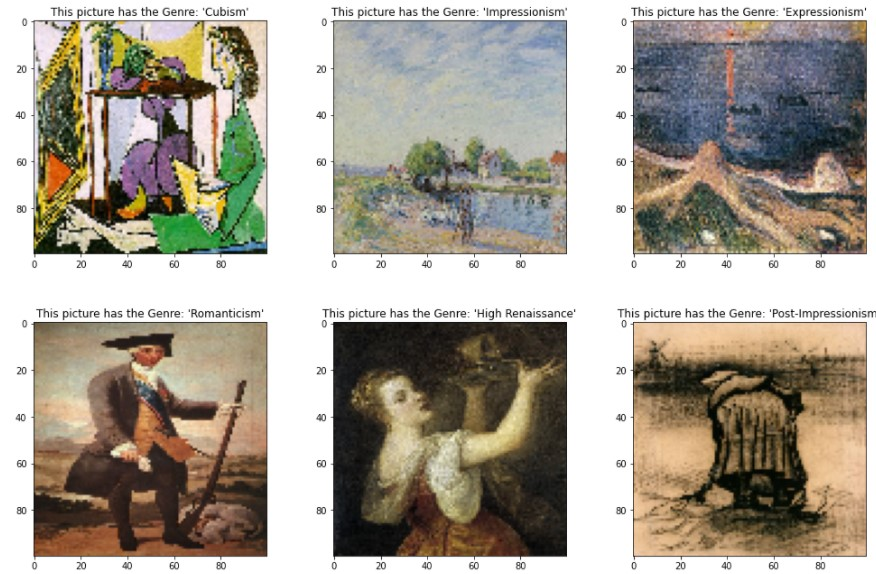
\includegraphics[width=0.7\textwidth]{content/data/beispiel.JPG}
    \caption{Einige Beispiel Bilder aus dem Testdatensatz, die in selber Form an das Netzwerk übergeben werden.}
    \label{fig:beispiel_bilder}
\end{figure}
\FloatBarrier
Da die Genre im Datensatz auf Englisch waren haben wir weiter mit den Englischen Genre Titlen gearbeitet.
Außerdem wurden, wie in dem Bild links unten in Abbildung \ref{fig:beispiel_bilder} zu sehen, manche Bilder durch das Ändern der Größe der Bilder, stark gestreckt oder gestaucht.
Zudem wird die Auflösung der Bilder durch das Ändern ihrer Größe schlechter.
Diese Limitierungen kommen durch die nur begrentzte Rechenleistung die uns zur Verfügung stand.
\subsection{Daten Aufbereitung}
Die Daten sind allerdings noch nach dem Aussortieren der Genre mit weniger als 200 Bildern sehr ungleich verteilt, wie in Abbildung \ref{fig:verteilung_daten} zu sehen ist.
So hat das Genre mit den meisten Vertretern über 1400 Bilder, wohingegen das Genre mit den wenigsten Bilder nur 260 Bilder hat.
\begin{figure}
    \centering
    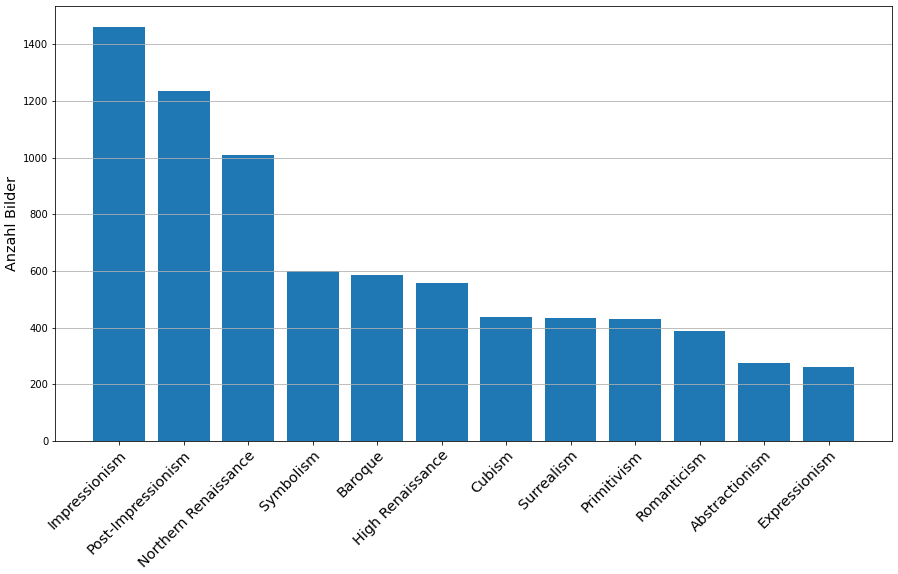
\includegraphics[width=0.55\textwidth]{content/data/Verteilung_Daten_Preprocessesing.PNG}
    \caption{Die Verteilung der Anzahl der Bilder nach Einlesen der Gerne mit mehr als 200 Bildern.}
    \label{fig:verteilung_daten}
\end{figure}
\\\\
Aus diesem Grund wurde nachdem die Daten in einen Test- und einen Trainingssatz aufgeteilt worden sind ein "Oversampling" und ein "Undersampling" durchgeführt.
Es wurden also zunächst $30\, \%$ der Bilder für den Testsatz und $70\, \%$ der Bilder für den Trainingssatz reserviert.
Es wird im späteren Verlauf weiter darauf eingegangen warum die Trennung in Test und Trainingssatz zuerst vorgenommen wurde.
\\\\
\subsubsection{Oversampling des Traingssatzes}
Wie bereits erwähnt wurde mit den Trainingssatz und dem Testsatz ein "Oversampling" und ein "Undersampling" durchgeführt.
Bei dem Oversampling wird dabei der Datensatz erweitert.
Dies wurde erreicht, indem zunächst die Anzahl von Bildern in dem Genre mit den meisten Bildern ermittelt wurde.
Im Testsatz waren dies 1023 Bilder.
Nun wurden die Bilder aus allen Genre die weniger als 1023 Bilder hatten kopiert und an das ursprüngliche Genre angehängt.
Dieser Prozess wurde für jedes unterbesetzte Genre so lange durchgeführt bis das jeweilige Genre auch 1023 Bilder hatte.
Das Ergebnis des "Oversampling" ist in Abbildung \ref{fig:oversampling} zu sehen.
Auf diese Weise tauchen in dem Datensatz, besonders in den Genre mit vorerst wenig Bildern, Bilder mehrfach auf.
Allerdings wird dadurch auch erreicht, dass die Verteilung der Anzahl der Bilder pro Genre gleich ist.
Dadurch kann das Netzwerk besser verallgemeinern.
Denn wenn der Datensatz eine ungleiche Anzahl von Bildern pro Genre haben würde, würde das Netzwerk diese Ungleichheit lernen und beim Testen zum Großteil das Genre "raten", welches im Traingssatz am häufigsten vorkam.
Dies ist natürlich unerwünscht, da das Netzwerk auf verschiedene Datensätze anwendbar seien soll, die Bilder aus den 12 gewählten Genre enthalten.
\begin{figure}
    \centering
    \caption{Ein Balkendiagramm welches die Anzahl der Bilder pro Genre zeigt. Links ist dabei der Traingssatz nach dem "Oversampling" und rechts der Traingssatz nach dem "Undersampling".}
    \begin{subfigure}{0.450\textwidth}
        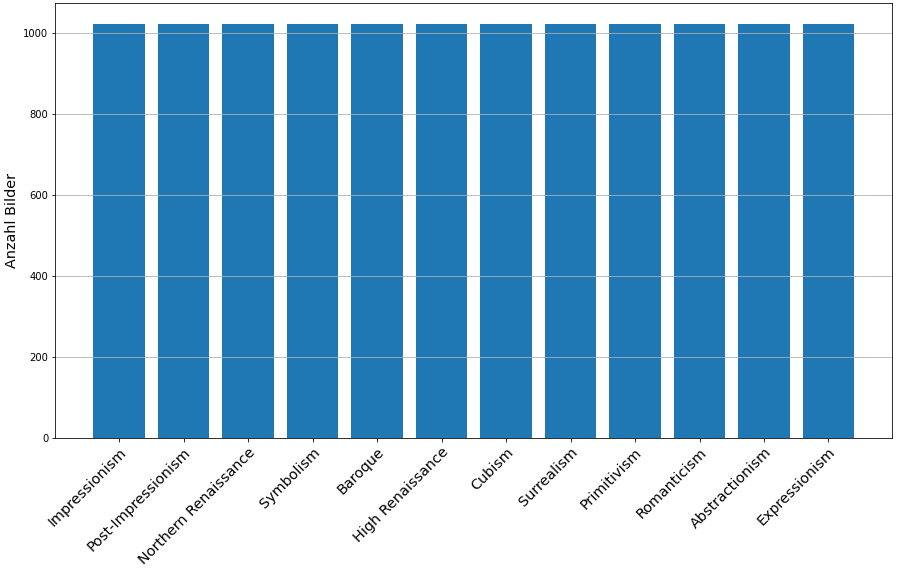
\includegraphics[width=\linewidth]{content/data/oversampling.PNG}
        \caption{Die Anzahl der Bilder nach dem "Oversampling" beträgt für jedes Genre im Traingssatz 1023.}
        \label{fig:oversampling}
    \end{subfigure}\hfil % <-- added
    \begin{subfigure}{0.450\textwidth}
        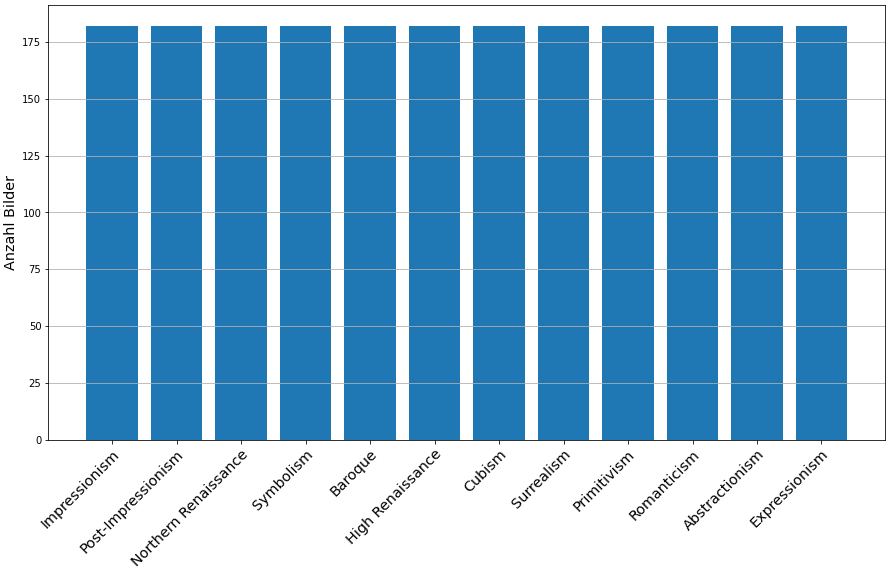
\includegraphics[width=\linewidth]{content/data/undersampling.PNG}
        \caption{Die Anzahl der Bilder nach dem "Undersampling" beträgt für jedes Genre im Traingssatz 182.}
        \label{fig:undersampling}
    \end{subfigure}\hfil % <-- added
    \label{fig:sampling}
\end{figure}
\\\\
\subsubsection{Undersampling des Traingssatzes}
Im "Undersampling" wird hingegen zum "Oversampling" der Datensatz an das Genre mit der geringsten Anzahl an Bildern angepasst.
Auf diese Anzahl wird die Anzahl der Bilder in jedem anderen Genre verringert.
Dabei werden Bilder aus dem Traingssatz gelöscht bis jedes Genre nur noch die entsprechende Anzahl an Bildern hat.
In unserem Fall hatte das Genre mit den wenisgten Bildern 182 Bilder.
Nach dem "Undersampling" hat also jedes Genre nur noch 182 Bilder.
Das Ergebnis des "Undersampling" ist in Abbildung \ref{fig:undersampling} zu sehen.
Auf diese Weise wird ebenfalls erreicht, dass die Anzahl alle Bilder in den verschiedenen Genre gleich ist.
Allerdings hat dies auch zur Folge, dass viele Bilder verloren gehen.
Da wir aber im vorhinein nicht sagen konnten welcher Traingssatz mit unserem Neuronalen Netzwerk bessere Ergebnisse liefert haben wir zunächst einen Traingssatz mit "Undersampling" und "Oversampling" erstellt.
\\\\
Sowohl der Traingssatz nach dem "Undersampling" als auch der Traingssatz nach dem "Oversampling" wurden nachdem sie erstellt wurden durchgemischt.
Dies geschieht, da sonst alle Bilder eines Genre aufeinander folgen.
Würden die Bilder also nicht gemischt werden, hätte das zur Folge, dass das Neuronale Netzwerk auch die Reihenfolge der Bilder trainiert, was zur Anwedung auf zufällige Bilder nicht erwünscht ist.

\subsubsection{Testdatensatz}
Als nächstes wurde der Testsatz bearbeitet.
Für diesen wurde nur ein "Undersampling" durchgeführt, da wir nicht wollten, dass sich in dem Testdatensatz Bilder doppelt befinden.
Nach dem "Undersampling" befanden sich im Testsatz noch 78 Bilder pro Genre.

\subsection{Das Convolutional Neural Network}
Zur Ermittlung der Genre aus den Bilddaten haben wir uns für ein "Convolutional Neural Network" (CNN) entschieden.
Der Vorteil an einem CNN ist, dass es Bildstrukturen lernt, was für unsere Problemstellung gut geeignet ist.
In Abbildung \ref{fig:model} ist der Finale Aufbau unseres Netzwerkes zu sehen.
Die Hyperparameter des Netzwerkes wurden bereits durch eine Rastersuche optimiert und sind in Abbildung \ref{fig:model_code} zu sehen.
Diese wurde für die Filter Anzahl der Convolutional Ebenen, die Größe des Kernels der Convolutional Ebenen, die Ausfallrate der Dropout Ebenen und die Anzahl der Neuronen in den dichten Ebenen und durchgeführt.
Die Ergebnisse der Rastersuche wurden anschließend in einem weiteren Jupyter Notebook abgespeichert um sie, wenn nötig, aufrufen zu können.
\\\\
Das optimierte Model aus Abbildung \ref{fig:model} besteht aus vier Convolutional Ebenen, die jeweils von einer Dropout Ebene und einer Pooling Ebene gefolgt werden.
Die Dropout Ebenen verhindern dabei die Überanpassung des Netzwerkes auf dem Traingssatz.
Auch die Pooling Ebenen verhindern die Überanpassung und ermöglicht es dem Netzwerk robuster gegen Rotationen von Bildern zu werden, was für Abstrakte Bilder vorteilhaft ist.
Außerdem reduziert es die Datenmenge was das Netzwerk schneller macht.
Nach der letzten Convolutional Ebene werden die Daten von der drei dimensionalen Matrix in eine ein dimensionalen Matrix übergeführt.
Darauf folgt eine weitere Dropout Ebene und eine dichte Ebene, die zur Reduzierung der Größe der Matrix genutzt wurde.
Abgeschlossen wird das Model durch eine dichte Ebene mit 12 Neuronen welche die Vorhersagen für die jeweiligen Bilder ausgibt.
Diese letzte dichte Ebene nuzt die \textit{softmax} Funktion als Aktivierungsfunktion, da sie einen Wertebereich zwischen 0 und 1 hat und so für die Ausgabe geeignet ist.
Die anderen Ebenen nutzen die \textit{ReLU} Funktion als Aktivierungsfunktion, aus dem Grund, dass diese keine Probleme mit schwindenen Gradtienten verursacht und sie des weiteren das Training sehr effizient macht.
Als Verlust Funktion wird die kategorische Kreuzentropie mit der Metrik Genauigkeit genutzt.
Diese ist für Mehrklassen Kategorisierungs Probleme die gängiste Verlust Funktion weswegen auch wir uns für sie entschieden haben.
Für die Metrik Genauigkeit haben wir uns entschieden, da wir möglichst viele Bilder richtig erkennen wollen ohne dabei falsche Vorhersagen zu machen.
Als "Optimizer" wurde "adam" genutzt.
\begin{figure}
    \centering
    \caption{Der Aufbau des genutzten optimierten Models. Links die Ausgabe der Funktion \textit{summary} von der Bibliothek \textit{Tensorflow} \cite{tensorflow2015-whitepaper} und rechts die Implementierung des Models als Code.}
    \begin{subfigure}{0.40\textwidth}
        \centering
        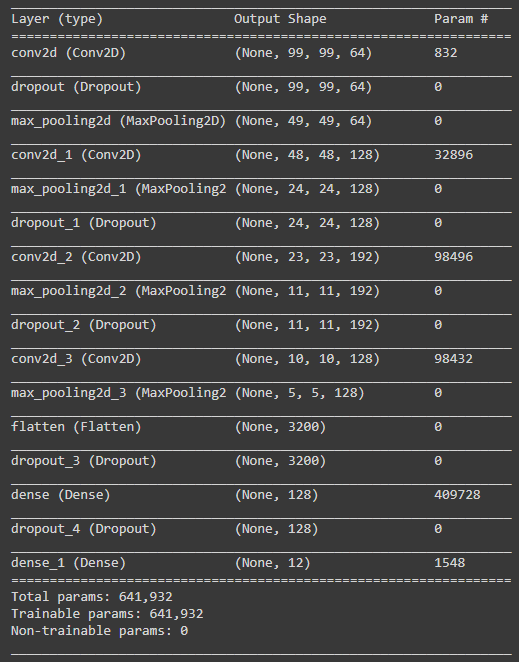
\includegraphics[width=0.6\linewidth]{content/data/model.PNG}
        \caption{Die Ausgabe der Funktion \textit{summary} auf das genutzte Model angewandt.}
        \label{fig:model_summary}
    \end{subfigure}\hfill
    \begin{subfigure}{0.40\textwidth}
        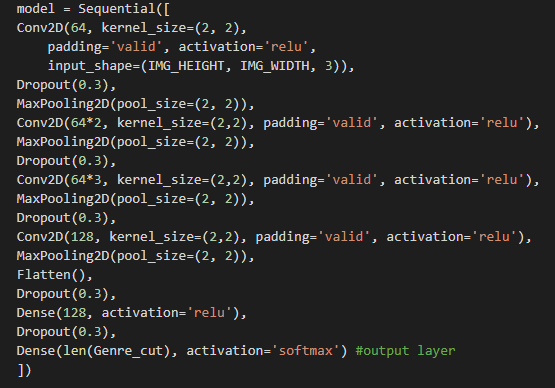
\includegraphics[width=\linewidth]{content/data/model_code.PNG}
        \caption{Die Code Implementierung des Models.}
        \label{fig:model_code}
    \end{subfigure}
    \label{fig:model}
\end{figure}
\\\\
Nachdem das Model erstellt wurde, haben wir es auf dem Trainingssatz welcher durch das "Oversampling" erweitert wurde trainiert.
Dazu haben wir einen Validierungssatz von $30\, \%$ der Trainingsdaten verwendet.
Zudem nutzen wir die Funktion \textit{EarlyStopping} aus \textit{Tensorflow} \cite{tensorflow2015-whitepaper}, um Überanpassung zu verhindern.
Wir haben mit einer maximalen Epochenzahl von 50 trainiert, \textit{EarlyStopping} hat aber nach der 35 Epoche abgebrochen.
Die Verlust Funktion des Models ist in Abbildung \ref{fig:loss} zu sehen.
Neben der Verlust Funktion ist zudem der Verlauf der Genauigkeit des Models über die 35 Epochen in Abbildung \ref{fig:accuracy} zu sehen.
Die beiden Plots wurden mit der Python Bibliothek \textit{matplotlib} \cite{matplotlib} erstellt.
Es ist zu erkennen, dass durch \textit{EarlyStopping} eine Überanpassung verhindert wurde.
Dies ist daraus zu schließen, dass sich die Funktionen auf den Validierungsdaten und auf den Trainingsdaten bei keinen der beiden Plots in Abbildung \ref{fig:training} in den letzten Epochen des Trainings weit voneinander entfernen.
\\\\
Es wurde auch ein Model auf den "Undersampling" Trainingsdaten durchgeführt.
Das so entstandene Model hat aber beim Testen wesentlich schlechter abegschnitten, weswegen im Weiteren nicht mehr weiter darauf eingegangen wird.
\begin{figure}
    \centering
    \caption{Der Verlauf der Verlust Funktion und der Genauigkeit über die 35 Trainingsepochen.}
    \begin{subfigure}{0.40\textwidth}
        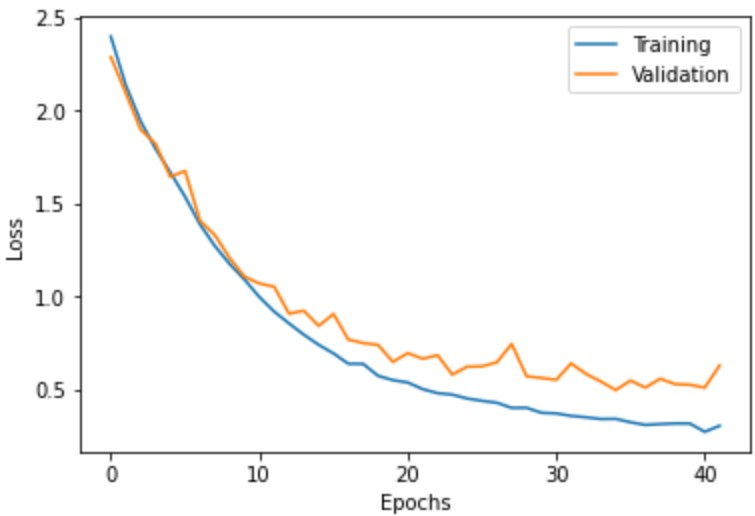
\includegraphics[width=\linewidth]{content/data/loss.JPG}
        \caption{Die Verlust Funktion des Models beim Traing über die 35 Epochen.}
        \label{fig:loss}
    \end{subfigure}\hfill
    \begin{subfigure}{0.40\textwidth}
        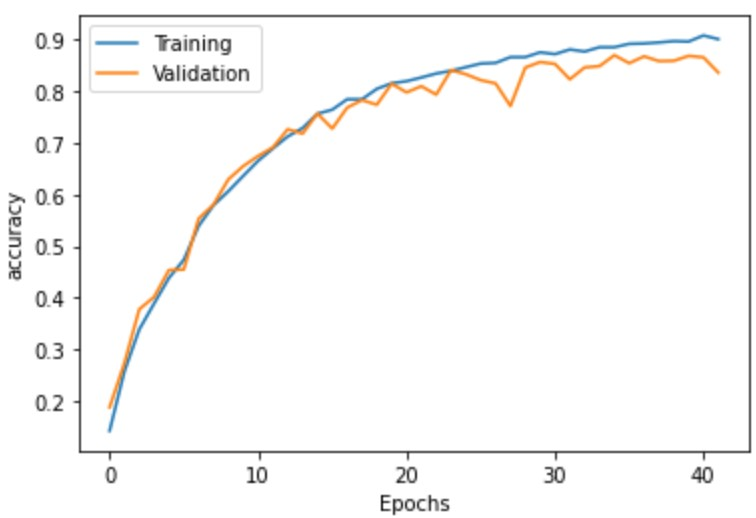
\includegraphics[width=\linewidth]{content/data/accuracy.JPG}
        \caption{Der Verlauf der Genauigkeit des Models beim Training über die 35 Epochen.}
        \label{fig:accuracy}
    \end{subfigure}
    \label{fig:training}
\end{figure}
Nach dem Trainieren sind wir direkt zum Testen übergegangen.
\section{Ergebnisse des Netzwerkes}
\label{sec:ergebnisse}
Das Model wurde nach dem Training auf den "Undersampling" Testdaten getestet.
Wir haben den "Undersampling" Satz genutzt, da wir vermeiden wollten doppelte Bilder im Testsatz zu haben.
Zudem brauchten wir eine Gleichverteilte Anzahl von Bilder pro Genre.
Der Testdatensatz hat so 78 Bilder pro Genre.
Mit dem genutzten Model konnten folgende Werte, auf den Testdaten, erziehlt werden
\begin{align*}
    \text{Genauigkeit} &= 48.18\, \% \\
    \text{Verlust} &= 2.36 \, .
\end{align*}
Um herauszufinden welche Genre am schlechtesten und am besten erkannt werden, haben wir zudem eine Konfusionsmatrix erstellt, welche in Abbildung \ref{fig:confusion} zu sehen ist.
\begin{figure}
    \centering
    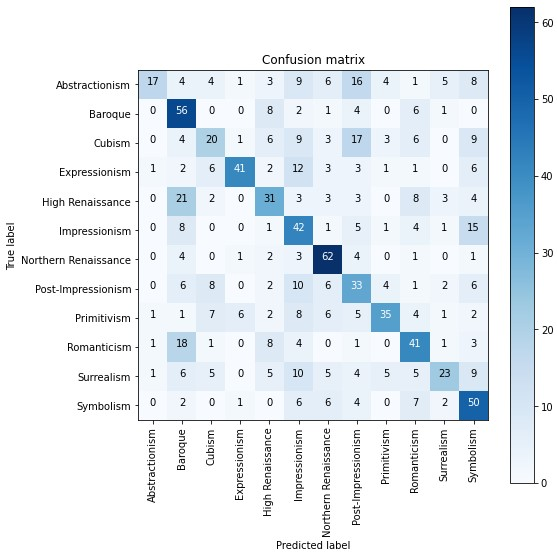
\includegraphics[width=0.5\textwidth]{content/data/confusion.JPG}
    \caption{Die Konfusionsmatrix zu den Testdaten mit dem genutzten Model.}
    \label{fig:confusion}
\end{figure}
Es lässt sich erkennen, dass besonders das Genre "Northern Renaissance" zu deutsch "Niederländische Renaissance" vom Model gut erkannt wird.
Dies ist damit zu begründen, das dieses Genre in dem genutzten Datensatz vorallem Bilder in schwarz-weiß enthält und so aus den anderen Bildern heraussticht.
Zudem verwechselt das Model am häufigsten "Hochrenaissance" Bilder (in der Abbildung mit "Highrenaissance" makiert) mit "Barock" Bilder (in der Abbildung mit "Baroque" makiert).
Wahrscheinlich liegt dies daran, dass beide Genre kräftige, kontrastreiche Farben nutzen und oft Menschen in Frontalansicht zeigen.
Um die falschen Vorhersagen des Models besser zu veranschaulichen wurden einige Bilder ausgegeben, dessen Genre falsch vom Model bestimmt wurden, diese sind in Abbildung \ref{fig:fehler} zu sehen.
Dabei steht "Predicted label" für die Vorhersagen des Models und "True label" für das wahre Genre des Bildes.
\begin{figure}
    \centering
    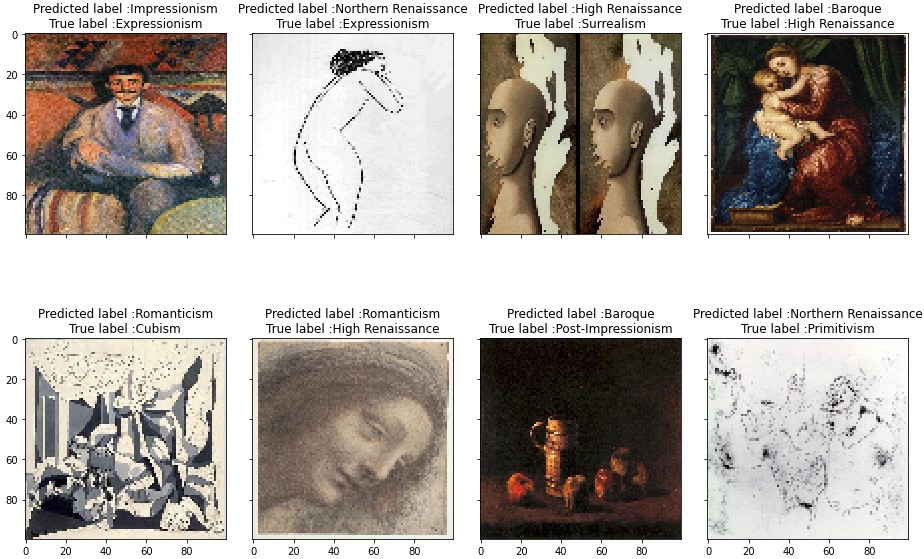
\includegraphics[width=\textwidth]{content/data/errors.JPG}
    \caption{Einige Bilder dessen Genre vom Model falsch bestimmt wurden.}
    \label{fig:fehler}
\end{figure}
Auch die falschen Vorhersagen sind bis auf einige Ausnahmen nachvollziehbar.
So sind in diesem Datensatz Bilder des Genre "Niederländische Renaissance" vor allem scharz-weiß, was die Abweichung in Bild 2 links oben und Bild 4 links unten erklärt.
Zudem ähnelt das Genre "Impressionismus" (in der Abbildung "Impressionism") von seiner Farbgebung und dem Stil sehr dem Expressionismus (in der Abbildung "Expressionism").
Wie bereits erwähnt nutzt das Genre "Hochrenaissance" (in der Abbildung mit "Highrenaissance" makiert) ähnliche Farben und Motive wie das Genre "Barock" (in der Abbildung mit "Baroque" makiert) wodurch die Verwechslung in dem Bild rechts oben zu begründen ist.
Die falsche Bestimmung des dritten Bildes von links oben kommt wahrscheinlich daher, dass in dem Bild ein menschlicher Kopf zu sehen ist, was ein typisches Motiv für die "Hochrenaissance" ist.
Woher die Abweichung der drei Bilder unten links stammen können wir allerdings nicht sicher sagen.
\section{Alternativmethode}
\label{sec:alternativ}
Bei der Alternativmethode haben wir uns für den k-nächste Nachbarn (KNN) Algorithmus entschieden.
Diesem übergeben wir drei Features die wir vorerst generieren.
Die drei Features sind pro Bild der Mittelwert der Pixelwerte, die Standardabweichung der Pixelwerte und der Mittelwert der Norm des Gradienten der Pixelwerte.
Wir haben uns dabei gedacht, dass durch den Mittelwert und die Standardabweichung erkannt werden kann ob ein Bild gleichmäßig in seiner Farbwahl ist oder nicht.
Durch den Mittelwert der Norm des Gradienten wollten wir ein Maß für die Stärke der Farbänderung haben.
Mit diesen drei Features trainieren wir den KNN auf den "Undersampling" Trainingssatz, da für das Trainieren mit den "Oversampling" Trainingsdaten die Rechenleistung nicht ausreichte.
Zudem denken wir, dass es für den KNN nicht Vorteilhaft gewesen wäre mit Daten zu trainieren die sich teilweise doppeln, da Dopplungen perfekte Nachbarn wären.
Der KNN erreicht auf dem "Undersampling" Testsatz folgende Genauigkeit
\begin{align*}
    \text{Genauigkeit} &= 15.00\, \%
\end{align*}
und schneidet damit wesentlich schlechter ab als das CNN.
In Abbildung \ref{fig:alternativ} ist die Konfusionsmatrix des KNN zu sehen.
\begin{figure}
    \centering
    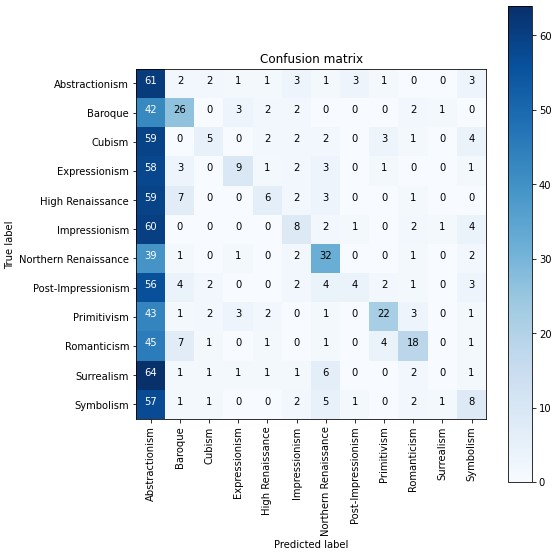
\includegraphics[width=0.5\textwidth]{content/data/alternativ.JPG}
    \caption{Die Konfusionsmatrix des KNN auf den Testdaten.}
    \label{fig:alternativ}
\end{figure}
Wie zu sehen ist sagt der KNN für fast jedes Bild das Genre "Abstrakte Expressionismus" (in der Abbildung "Abstractionism").
Wir sind uns leider nicht sicher, warum der KNN fast nur dieses Genre ausgibt.
Nur auf einigen Genre bestimmt der KNN etwa ein drittel der Bilder richtig.
Am zuverlässigsten tut er dies für die "Niederländische Renaissance" (in der Abbildung "Northern Renaissance"), da diese Bilder im genutzten Datensatz oft nur in scharz-weiß sind.

\section{Zusammenfassung}
Die erreichte Genauigkeit von $48.18 \, \%$ des CNN ist eine wesentlich höhere Genauigkeit als wir bei 12 Genre erwartet hätten.
Im Vergleich zu der Genauigkeit des KNN von nur $15 \, \%$ sagte das CNN wesentlich zuverlässiger das Genre der Bilder vorraus als der KNN.
Durch bessere Bildqualität und einen größeren Datensatz könnte wahrscheinlich diese Genauigkeit noch weiter gesteigert werden.
Da aber eine höhere Bildqualität eine höhere Pixelanzahl erfordert wäre der Datensatz schnell zu groß geworden um mit unseren Methoden verarbeitet werden zu können, da uns die Rechenleistung gefehlt hat. 
Zudem war es nicht optimal, das einige der Künstler*innen in mehreren Genre tätig waren und wir deswegen einigen Bilder des Datensatzes ein falschen Genre gegeben haben.
Denn uns hat die Zeit gefehlt um bei den besagten Künstlern*innen alle Bilder durch zu gehen und einzelnt zu entscheiden zu welchem Genre das Bild gehört.
Durch die falsche Etikettierung einiger Bilder ist die Genauigkeit des Models mit Sicherheit geringer geworden.
\\\\
Des weiteren ist der genutzte Datensatz für einige Genre nicht wirklich repräsentativ, da sich einige Genre zum größten Teil aus Bildern von nur einem Künstler*in zusammen setzten.
So besteht das Genre Post-Impressionismus zu über $71\,\%$ aus Bildern des Künstlers Vincent van Gogh.
Dies legt die Vermutung nahe, dass das Netzwerk bei einigen Genre eher den Stil eines bestimmten Künstlers*in erkennt, anstatt das Genre des Bildes.
Zu Umgehen wäre dieses Problem durch einen größeren Datensatz mit mehr Künstlern*innen pro Genre, die jeweils ähnlich viele Bilder geschaffen haben.
\\\\
Abschließend kann gesagt werden, dass das CNN zwar gute Ergebnisse liefert aber definitiv keinen Kunstkritiker*in ersetzt.
Dafür ist die Genauigkeit des Netzwerkes zu gering und die Kunst zu komplex.
Wobei dazu zu sagen ist, dass in den meisten Fällen Kunstkritikern*innen auch weitere Daten wie Erscheinungsdatum des Bildes und Nationalität des Künstlers*innen zu Verfügung stehen.
Durch diese könnte die Leistung des Netzwerkes ebenfalls verbessert werden, dies war allerdings nicht Teil unserer Problemstellung da wir allein aus den Bildern das Genre bestimmen wollten.

\section{Anhang}
\label{sec:anhang}

\begin{table}
    \centering
    \caption{Alle Künstler*innen die in der "artist.csv"-Datei enthalten sind, sowie die Genre die ihnen zugeordnet werden und die Anzahl von Gemälden die sie zu dem Grunddatensatz beitragen.}
    \begin{tabular}{l l c}
        \toprule
        Name & Genre & Anzahl der Gemälde \\
        \midrule
        Amedeo Modigliani   &   Expressionismus                   & 193    \\
        Vasiliy Kandinskiy  &  Abstrakte Expressionismus  &  88     \\
        Diego Rivera    &        Sozialistischer Realismus, Muralismo       &  70       \\
        Claude Monet    &        Impressionismus                   &  73      \\
        Rene Magritte   &       Surrealismus, Impressionismus      & 194        \\
        Salvador Dali   &       Surrealismus                      & 139       \\
        Edouard Manet   &       Realismus, Impressionismus & 90     \\
        Andrei Rublev   &       Byzantinische Kunst   & 99        \\
        Vincent van Gogh    &    Post-Impressionismus  & 877      \\
        Gustav Klimt    &        Symbolismus, Jugendstil   & 117     \\
        Hieronymus Bosch    &    Niederländische Renaissance    & 137      \\
        Kazimir Malevich    &    Suprematismus & 126      \\
        Mikhail Vrubel  &      Symbolismus   & 171        \\
        Pablo Picasso   &       Cubismus  & 439       \\
        Peter Paul Rubens   &   Barock & 141       \\
        Pierre-Auguste Renoir &  Impressionismus   & 336      \\
        Francisco Goya  &      Romantik & 291        \\
        Frida Kahlo &         Primitivismus, Surrealismus    & 120      \\
        El Greco    &            Manierismus   & 87       \\
        Albrecht Dürer  &      Niederländische Renaissance    & 328        \\
        Alfred Sisley   &       Impressionismus   & 259       \\
        Pieter Bruegel  &      Niederländische Renaissance    & 134        \\
        Marc Chagall    &        Primitivismues & 239      \\
        Giotto di Bondone   &  Protorenaissance   & 119       \\
        Sandro Botticelli   &   Frühe Renaissance   & 164       \\
        Caravaggio  &          Barock & 55     \\
        Leonardo da Vinci   &   Hochrenaissance   & 143       \\
        Diego Velazquez &     Barock & 128     \\
        Henri Matisse   &       Impressionismus, Post-Impressionismus  & 186        \\
        Jan van Eyck    &        Niederländische Renaissance    & 81       \\
        Edgar Degas &         Impressionismus   & 702     \\
        Rembrandt   &           Barock & 262       \\
        Titian  &              Hoch Renaissance, Manierismus    & 255     \\
        Henri de Toulouse-Lautrec &      Post-Impressionismus    & 81     \\
        Gustave Courbet    &   Realismus & 59     \\
        Camille Pissarro      &   Impressionismus, Post-Impressionismus  & 91       \\
    \bottomrule
    \end{tabular}
\end{table}

\begin{table}
    \centering
    \caption{Alle Künstler*innen die in der "artist.csv"-Datei enthalten sind, sowie die Genre die ihnen zugeordnet werden und die Anzahl von Gemälden die sie zu dem Grunddatensatz beitragen.}
    \begin{tabular}{l l c}
        \toprule
        Name & Genre & Anzahl der Gemälde \\
        \midrule
        William Turner      &   Romantik & 66        \\
        Edvard Munch          &   Symbolismus, Expressionismus   & 67      \\
        Paul Cezanne          &   Post-Impressionismus  & 47      \\
        Eugene Delacroix      &   Romantik & 31      \\
        Henri Rousseau      &   Primitivismus & 70        \\
        Georges Seurat      &   Post-Impressionismus  & 43        \\
        Paul Klee         &   Abstrakte Expressionismus, Surrealismus   & 188       \\
        Piet Mondrian        &   Neoplastizismus   & 84       \\
        Joan Miro         &   Surrealismus  & 102     \\
        Andy Warhol       &   Pop Art & 181     \\
        Paul Gauguin          &   Symbolismus, Post-Impressionismus  & 311      \\
        Raphael          &   Hochrenaissance   & 109      \\
        Michelangelo          &   Hochrenaissance   & 49      \\
        Jackson Pollock    &   Abstrakte Expressionismus  & 24     \\
        \bottomrule
    \end{tabular}
    \label{tab:artist}
\end{table}
\printbibliography{}

\end{document}
